\section{Results}
\label{sec:results} % Label for referencing

In this mini-challenge, our objective was to generate high-quality (HQ) face images from corrupted low-quality (LQ) ones using the Real-ESRGAN model. Below we present some example outputs along with the loss curves observed during training.

\begin{figure}[htbp]
    \centering
    \begin{minipage}{0.45\textwidth}
        \centering
        
\includegraphics[width=\textwidth]{imgs/output_00328.png}
        \caption{Example of HQ image generated from LQ input.}
        \label{fig:image1}
    \end{minipage}\hfill
    \begin{minipage}{0.45\textwidth}
        \centering
        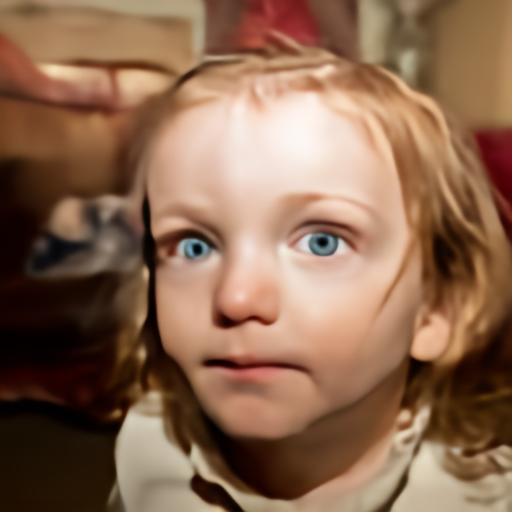
\includegraphics[width=\textwidth]{imgs/output_00386.png}
        \caption{Another example of enhanced HQ output.}
        \label{fig:image2}
    \end{minipage}
\end{figure}

\begin{figure}[htbp]
    \centering
    \begin{minipage}{0.45\textwidth}
        \centering
        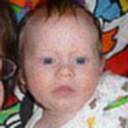
\includegraphics[width=\textwidth]{imgs/00328.png}
        \caption{Further illustration of HQ output from Real-ESRGAN.}
        \label{fig:image3}
    \end{minipage}\hfill
    \begin{minipage}{0.45\textwidth}
        \centering
        
\includegraphics[width=\textwidth]{imgs/00386.png}
        \caption{Additional HQ image showcasing model capabilities.}
        \label{fig:image4}
    \end{minipage}
\end{figure}

\begin{figure}[htbp]
    \centering
    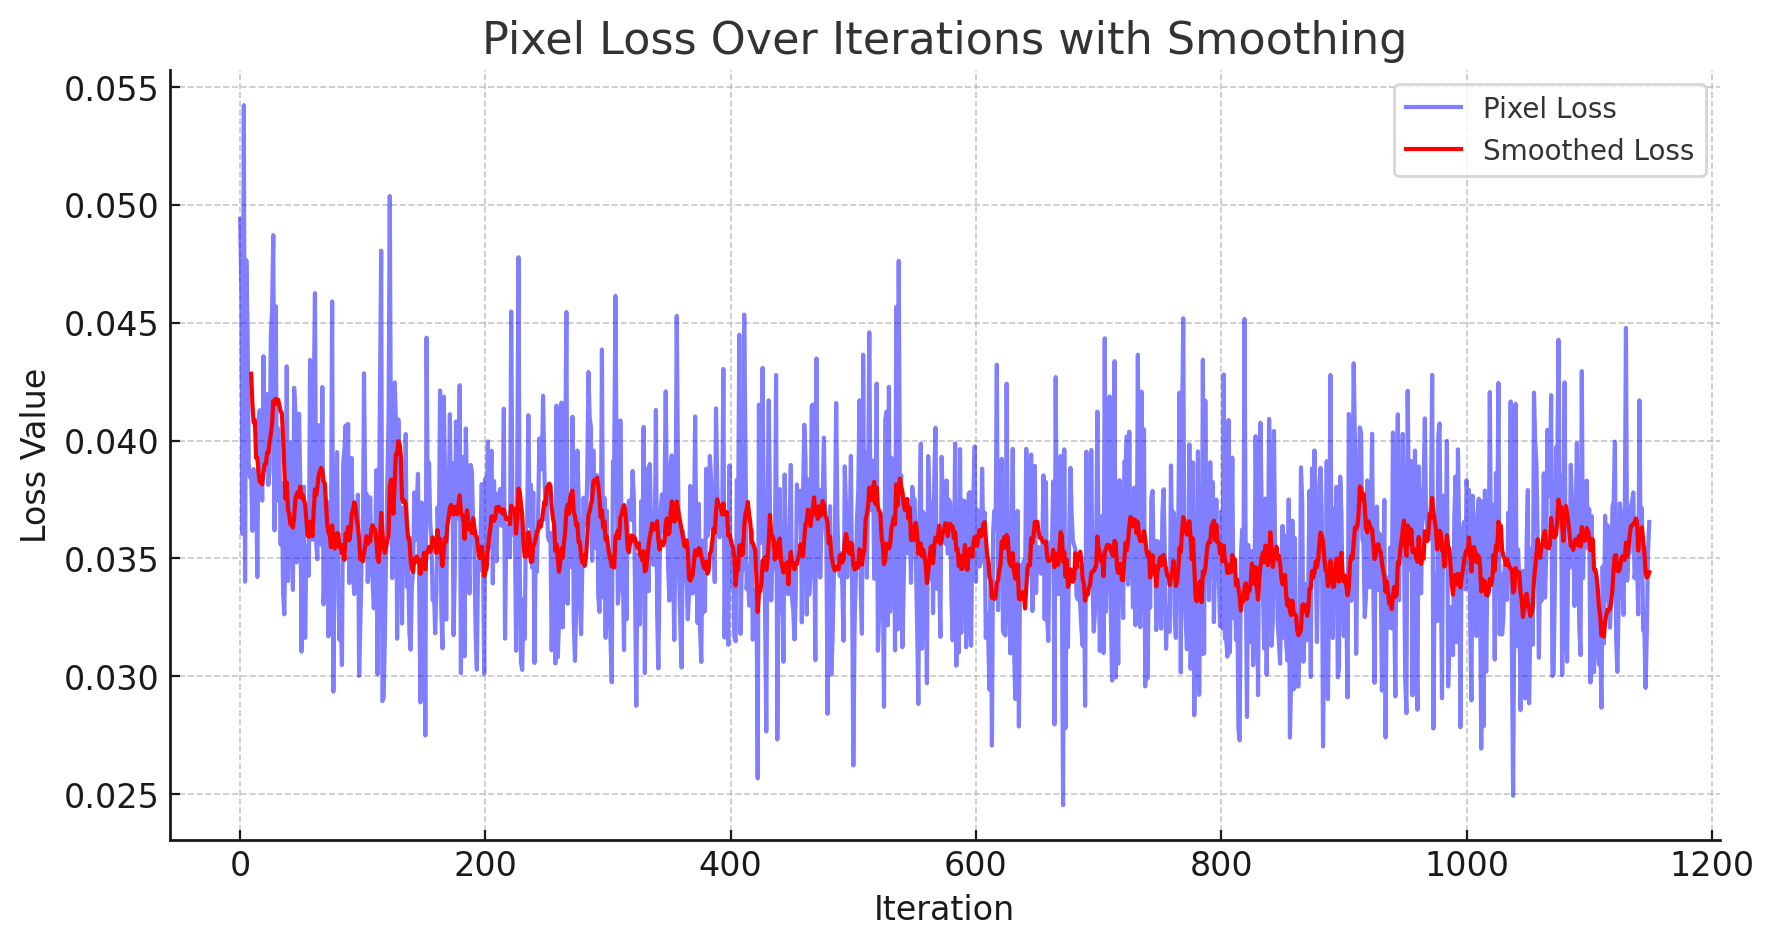
\includegraphics[width=\textwidth]{imgs/losses.png}
    \caption{Training loss curves over 115,000 iterations.}
    \label{fig:image5}
\end{figure}

These results were achieved after training the model on the NTU GPU cluster using an A40 GPU for 115,000 iterations—the maximum allowed training duration. The model reached a Peak Signal-to-Noise Ratio (PSNR) score of $26.40953$ in the blind test, demonstrating the effectiveness of the Real-ESRGAN model in enhancing image quality from LQ inputs. Detailed settings used during the training are provided in the appendix.
